\documentclass{acmsig}
\usepackage[color=yellow,obeyFinal]{todonotes}
\usepackage{graphicx}
\usepackage{epstopdf}
\usepackage{float}
\usepackage{varioref}
\usepackage{mathtools}
\usepackage{xspace}
\usepackage{subfigure}
\usepackage{hyperref}
\usepackage{balance}
\usepackage{algorithm}
\usepackage{algpseudocode}
\usepackage{paralist}
\usepackage{cite}
\usepackage[T1]{fontenc}
\usepackage{beramono}
\usepackage{listings}
\usepackage{xcolor}

\definecolor{dkgreen}{rgb}{0,0.6,0}
\definecolor{gray}{rgb}{0.5,0.5,0.5}
\definecolor{mauve}{rgb}{0.58,0,0.82}

\lstdefinestyle{myScalastyle}{
  frame=tb,
  language=scala,
  aboveskip=3mm,
  belowskip=3mm,
  showstringspaces=false,
  columns=flexible,
  basicstyle={\small\ttfamily},
  numbers=none,
  numberstyle=\tiny\color{gray},
  keywordstyle=\color{blue},
  commentstyle=\color{dkgreen},
  stringstyle=\color{mauve},
  frame=single,
  breaklines=true,
  breakatwhitespace=true,
  tabsize=3,
}

\newcommand{\etal}{\textit{et al.}\xspace}
\newcommand{\eg}{\textit{e.g.}\xspace}
\newcommand{\ie}{\textit{i.e.}\xspace}
\newcommand{\etc}{\textit{etc.}\xspace}
\newcommand{\vs}{\textit{vs.}\xspace}
\newcommand{\keyval}{$\langle\text{key}, \text{value}\rangle$\xspace}
\DeclarePairedDelimiter\floor{\lfloor}{\rfloor}

\newcommand{\noteby}[2]{\todo[inline]{#2\hspace*{\fill}\mbox{ --#1}}}

%========================================================
\newcommand\mytodo[1]{\textcolor{red}{[#1]}}

\makeatletter
\def\BState{\State\hskip-\ALG@thistlm}
\makeatother

\usepackage{caption}
%========================================================

% correct bad hyphenation here
\hyphenation{op-tical net-works semi-conduc-tor}

\begin{document}

% paper title
% can use linebreaks \\ within to get better formatting as desired
\title{In-memory Cache-based Work Sharing for Large-scale Distributed Systems}


% author names and affiliations
% use a multiple column layout for up to three different
% affiliations
\numberofauthors{3}
\author{
\alignauthor
Khoa Nguyen\\
       \affaddr{EURECOM}\\
       \email{nguyentr@eurecom.fr}
\alignauthor
Hung Phan\\
       \affaddr{EURECOM}\\
       \email{phan@eurecom.fr}
\alignauthor 
Pietro Michiardi
       \affaddr{EURECOM}\\
       \email{michiard@eurecom.fr}
}
% make the title area
\maketitle

\begin{abstract}
In collaborative large-scale distributed systems, analytical jobs submitted by various users often share similar work, for example scanning and processing the same set of data. Instead of optimizing jobs independently, which results in redundant and wasteful processing, many well-known multi-query optimization techniques could be employed to save a considerable amount of cluster resources. In this work, we introduce a novel idea of applying cache primitives and multi-query optimization means to large-scale distributed systems. By exploiting the shareable common and similar subexpressions along with leveraging the full potential power of the distributed memory cache, our system - Spark SQL Server transforms a batch of input queries into a new more efficient one which avoids unnecessary computations. One major challenge is that we need to take into account the memory constraint and important properties of the distributed memory cache. In order to find the near optimal execution plan, the optimizer must trade off between performance boost and memory consumption in a cost-based fashion. Extensive experiments in our system show significant benefit in both the micro-benchmarks and the workloads consisting of queries in the TPC-DS benchmark.
\end{abstract}

%%%%%%%%%%%%%%%%%%%%%%%%%%%%%%%%%%%%%%%%%%%%%%%%%%%%%%%%%%%%%%%%%%%%%%%%%%%%%%%
\section{Introduction}
\label{sec:introduction}
Nowadays, more and more e-commerce companies have been embracing new technologies to cope with the huge expansion of their data. Big data analytics helps ones gain insights into the market as well as drive to rational business decisions. General-purpose cluster processing frameworks such as MapReduce \cite{dean2008mapreduce}, Dryad \cite{isard2007dryad} and Spark \cite{zaharia2012resilient} were developed to address those needs. Moreover, built on top of those, high-level SQL-like languages (Pig, DryadLINQ, Spark SQL respectively) have been gaining popularity, due to their simple and declarative nature together with rich automatic optimization.

In shared large-scale distributed systems, analytics jobs submitted by various users often share similar work, for example scanning and processing the same set of data. However, most prevalent query optimizers focus on finding an optimal plan for each job. Instead of optimizing them independently, which results in redundant and wasteful processing, many well-known multi-query optimization techniques could be employed to save a considerable amount of cluster resources. One typical instance is the research in \cite{gunda2010nectar} on 25 production clusters, estimated that over 35,000 hours of redundant computation can be eliminated per day by caching intermediate results (approximately equivalent to shutting off 1500 machines daily).

Some high-level languages support multiple query optimization, for example Pig and Spark SQL. However this feature is not achieved automatically and only available for single user. In Pig, users manually specify which data should be shared by using the ``Split" operator. In Spark SQL, users can explicitly invoke ``Cache" or ``Persist" operation on a DataFrame (a query) to keep the result in memory for later access. In fact, deciding by hand the best data to cache (materialize to RAM) might be a problematic task that is usually done by data experts. A better optimizer should use its knowledge to solve this task efficiently.

Established automatic solutions, for example the studies in similar subexpressions sharing \cite{zhou2007efficient} and materialized views selection \cite{goldstein2001optimizing, mistry2001materialized}, were proposed for RDBMSes. The idea of reusing intermediate data across queries or jobs in distributed environment has also received a significant body of research  recently: for MapReduce \cite{mrshare, mqo}, for SCOPE operating on top of Cosmos \cite{silva2012exploiting} and for Massive Parallel Processing (MPP) framework \cite{el2015optimization}. We will discuss these state-of-the-art studies in more detail in Section \ref{sec:related}. Applying multi-query optimization ideas into contemporary large-scale data analytic framework raises new challenges due to its scalability and distributed nature.

In this paper, we devise a different principle to achieve work sharing - in-memory cache primitives. By exploiting the shareable common or similar subexpressions and leveraging the full potential power of the distributed memory cache, our system - Spark SQL Server transforms a batch of SQL-like input queries into a new more efficient one which avoids unnecessary computations and reduces query processing cost. Notably, caching technique has recently gained attention in the research community, and many systems now implement some form of memory-backed storage \cite{tachyon, hdfs}.

Our optimization strategy begins with identifying the sharing opportunities: detect and exploit Similar subExpressions (SEs). SEs are identical or similar expressions that appear more than one in a query or in multiple queries submitted as batch. For example the common table expressions, which are defined once and referred multiple times in a query, are also SEs. Detected SEs should be executed only once by rewriting some queries to use Covering subExpression(s) (CEs). A CE, being constructed from a group of SEs, produces all common sharing tuples for the queries using it. We refer those queries as the \emph{consumers} of that CE. A CE will then become a \emph{cache plan} if it is chosen to be included in the final execution plan. The system ensures that \emph{cache plans} are computed only once and materialized in RAM so that later jobs can benefit from them. Due to the limited availability of cluster's memory, our objective of \emph{cache plans} selection is to minimize the total query processing under a given memory constraint. We modeled this dilemma as the Multiple-choice Knapsack problem and solved it using some heuristics and cost estimation. To the best of our knowledge, our approach is the first that could exploit the in-memory distributed caching to achieve high performance work sharing.

We summarize our main contributions:
\begin{enumerate}
	\item We believe that ours is the first paper that systematically explores how to apply multi-query optimization techniques along with the distributed in-memory cache to achieve high performance work sharing in distributed environment.
	\item We solve the optimization problem by building an optimizer as an extension for Spark SQL operating on top of the Spark engine. The optimizer avoids generating obviously bad plans as early as possible.
	\item We propose a general and abstract cost model, based on pre-computed statistics information, capable of estimating the efficiency of different plans and produce a globally near optimal execution plan.
	\item We extensively experiment on our prototype and demonstrate interesting characteristics and prospect for a high performance work sharing system for large-scale distributed environment.
\end{enumerate}

The rest of the paper is structured as follows:  Section \ref{sec:related} covers related work on multiple query optimization in traditional database management systems and cluster computing engines. We then introduce and formalize our optimization problem in Section \ref{sec:problem}. The overview on the idea of using cache primitives to achieve high performance for distributed system is discussed in Section \ref{sec:caching}. In Section \ref{sec:implementation}, we provide the implementation details of our idea for Apache Spark and Spark SQL. We evaluate the performance of our proposed approach in Section \ref{sec:evaluation}. Finally, we conclude the paper in Section \ref{sec:conclusion}.
%%%%%%%%%%%%%%%%%%%%%%%%%%%%%%%%%%%%%%%%%%%%%%%%%%%%%%%%%%%%%%%%%%%%%%%%%%%%%%%

%%%%%%%%%%%%%%%%%%%%%%%%%%%%%%%%%%%%%%%%%%%%%%%%%%%%%%%%%%%%%%%%%%%%%%%%%%%%%%%
\section{Related Work}
\label{sec:related}
The multi-query optimization (MQO) is well-known as the technique of minimizing the total execution time by performing common tasks only once. In this paper, we systematically propose a comprehensive solution for large-scale distributed computing engines; that combines the in-memory caching primitives with the state-of-the-art MQO techniques: similar subexpressions sharing, materialized view selection and work-sharing.

% similar subexpressions & materialized views
\emph{\textbf{MQO in RDBMSes.}} Similar subexpressions sharing has been well studied by Zhou et al. in \cite{zhou2007efficient}. As was pointed out, to improve query performance, common subexpressions could be evaluated once and the result is reused in multiple places. His solution could avoid some limitations of earlier work \cite{finkelstein1982common, roy2000efficient} by (i)considering all generated plans as sharing opportunities to avoid leading to suboptimal plans and (ii) also considering multiple competing covering expressions. 

%The proposed solution has 3 steps: (1) Table signature generation, (2) Generation of candidates CSEs and (3) Optimization with candidate CSEs.

% Differences:
% Table signature to identify
% heuristic to prune bad candidates
% Covering expression candidates are evaluated in cost-based manner (same), but: they already have their own cost estimation
% not use in-memory caching
% Plans are stored in MEMO structure

Materialized views can be used is conjunction with MQO to speed up query performance. It relies on the fact that accessing to a materialized view can be much faster than recomputing it. Nevertheless, due to the nature of RDBMSes, base relation changes frequently leading to cache invalidation and view maintenance cost. In this paper, we will concentrate on big data analytics queries in which the input data is usually stable in the Distributed File System (DFS). Additionally, while materialized views are usually materialized permanently (to disk), our approach considers temporarily materializing common shareable data to RAM as a mean to boost the overall jobs' performance.

% work-sharing & MQO in MapReduce + MQO in Cloud & MPP
\emph{\textbf{MQO in Cloud and MPP.}} Inheriting from the MQO techniques in RDBMSes, Silva et al. \cite{silva2012exploiting} proposed an extension to the SCOPE query optimizer which optimizes cloud scripts containing common expressions while reconciling the physical requirements.

In the context of Massively Parallel Processing databases, The work in \cite{el2015optimization} presents a comprehensive framework for the optimization of Common Table Expressions (CTEs) implemented for Orca (the Pivotal Query Optimizer). Compared to our method, we not only consider CTEs but also similar subexpressions as the potential sharing opportunities. We achieve work-sharing by utilizing the distributed memory cache, not by materializing intermediate result to disk.

\emph{\textbf{MQO in MapReduce.}} The idea of avoiding redundant processing by batching the queries and make them share some intermediate results was widely studied in \cite{mrshare, mqo, agrawal2008scheduling, bhatotia2011incoop, elghandour2012restore, silva2012exploiting, li2011platform, li2012scalla}. Typically among them, MRShare \cite{mrshare}, is a sharing framework for MapReduce that first identifies different jobs sharing portions of identical work. These jobs are then transformed into a compound job such that \emph{scan sharing}, \emph{Map Output sharing} and \emph{Map Functions Sharing} could be achieved. While MRShare focuses on sharing between queries that are executed concurrently, ReStore \cite{elghandour2012restore}, as an extension on higher level language - Pig, allows jobs submitted at different time share the results. By keeping intermediate data and then reuse them in future jobs, the performance of the whole workflows improves. They both modifies the internal process of the computing engine, we don't. Our system is an extension to the current Spark SQL optimizer (the Catalyst \cite{sparksql}).

None of earlier work comprehensively take into account the usage of the distributed memory to achieve high performance work sharing.

%Coming to the ``big data'' era, where both volume, velocity and the variety of structure of data are increasingly %high, integrating optimization ideas from traditional DBMSes to distributed environment is a nontrivial task. It %requires modifications and considerations on new aspects, such as network cost and physical parallel computation.

% . Early work on multi-query optimization [] focused primarily on exhaustive algorithms, considering sharing %opportunities only among the best plans for each query, leading to suboptimal solution. [] constructs covering %expression to cover all its potential consumers, which may result in producing too much data, as pointed in [].
%%%%%%%%%%%%%%%%%%%%%%%%%%%%%%%%%%%%%%%%%%%%%%%%%%%%%%%%%%%%%%%%%%%%%%%%%%%%%%%

%%%%%%%%%%%%%%%%%%%%%%%%%%%%%%%%%%%%%%%%%%%%%%%%%%%%%%%%%%%%%%%%%%%%%%%%%%%%%%%
\section{Problem Statement}
\label{sec:problem}
We discuss the optimization opportunities and challenges through the following example. We also provide the readers a more practical example of queries taken from the TPC-DS benchmark \cite{tpcds} in Section \ref{sec:tpcds-sharing}.

\begingroup
\fontsize{8pt}{9pt}
\selectfont
\begin{verbatim}
QUERY 1:
SELECT name, dept_name, salary
FROM employees, departments, salaries
WHERE dep = dept_id
	AND id = emp_id
	AND gender = 'F'
	AND location = 'us'
	AND salary > 20000
ORDER BY salary DESC

QUERY 2:
SELECT name, dept_name, title, 
	to as title_expired_on
FROM departments, employees, titles
WHERE dep = dept_id
	AND id = emp_id
	AND gender = 'F'
	AND location = 'us'
	AND from >= 2010

QUERY 3:
SELECT id, name, salary, from_date
FROM employees, salaries
WHERE id = emp_id
	AND age > 30
	AND SALARY > 30000
\end{verbatim}
\endgroup

\begin{figure*}[htbp]
	\centering
	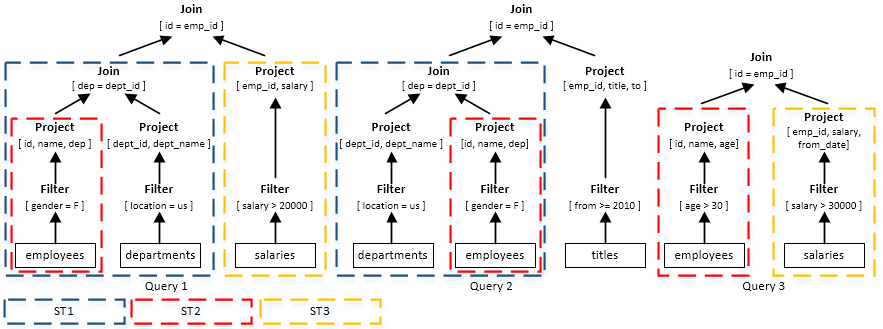
\includegraphics[scale=0.65]{figures/common_sub}
	\caption{Optimized operator trees} 
	\label{fig:common_sub}
\end{figure*}

Looking at the \emph{FROM} statements above, we can see that 3 queries (jobs) can share the common reading of \textbf{employees}, \textbf{departments} and \textbf{salaries} tables. Although disk speed has increased recently, a possible optimization would be to avoid wasteful disk I/O. Indeed, I/O operations are heavyweight because they not only involve reading records from file, but also parsing and transforming those into objects in memory for processing. What if we could tell the first job to \emph{cache} the input data after reading it, so that the later jobs do not have to ``waste time'' doing redundant I/O operations? A more refined approach could be to find common work (similar subexpressions) among these queries (for instance reading input, filtering and projecting records, joining tables, etc.) so that we can assure we are ``maximizing'' sharing benefit while ``minimizing'' the cache size (memory utilization).

To facilitate reader's understanding, we use Figure \ref{fig:common_sub} which illustrates the optimized operator trees (optimized logical plans) of 3 queries in the above example. Those optimized logical plans are produced by Spark SQL's query optimizer that will be next translated into physical plans for execution. The leaf nodes represents the base relations. Each intermediate node is a relational algebra operator (Filter, Project, Join, etc.). The arrows indicate data flow.

As can be seen from Figure \ref{fig:common_sub}, multiple SEs can be identified. They have the same tree structure but different filtering predicates and projections, for example the similar subexpression 2 (SE2): $Project_p(Filter_f(employees))$ which appears in both 3 queries. We can save some reading, parsing, filtering and projecting costs on the \textbf{employees} table 2 times out of 3. In order to achieve that, a CE will be constructed by ``combining'' operators' predicates: \[Project_{id, name, dep, age, gender}(Filter_{gender=F \cup age>30}(employees))\]

Constructing the CE in this way makes its output can be used to answer the consumer queries. By executing this CE and keeping the result in memory, the consumers can retrieve that data instead of reading and computing again from scratch. Thereby, the query execution time reduces significantly. Imagine that the Projection operator only projects on 5 out of total 10 columns and the Filtering keeps 60\% of records in \textbf{employees} tables, then the consumers rather than re-read and scan the whole table from disk, they can just extract from a smaller chunk of cached data in-memory. 

In the same way, the SE3 and SE4 share the projection and filtering on \textbf{deparment} and  \textbf{salaries} tables respectively. Note that sharing some SEs is always better than some others, for instance the SE $Project_p(Filter_f(employees))$ does more computations but produces less or equal output data than the smaller SE - $(Filter_f(employees))$. That's why our identification algorithm does not take into account the obvious worse SE.

Between Query 1 and Query 2, the SE1, which not only involves projections and filterings on tables but also joining, may become a better sharing option comparing to SE2 and SE3. Greater SEs are more favoured in general, however, what if the \emph{Join} operator produces a large amount of data that is too expensive to \emph{cache} under a limited amount of memory? Data caching in memory can be a costly operation, especially in distributed environment. Our study shows that blindly caching data may lead to higher costs of job execution. One next problem we may have to face is to select multiple CEs that will later become \emph{cache plans} such that the job's performance is maximized while the memory consumption condition is satisfied.

Hence, the problem we attempt to solve in this paper can be described as follows: Given a batch of queries submitted, transform it into a more efficient batch such that the new batch results in shorter aggregate job running time, taking into account the memory constraint and extra computations. Particularly in this work, we develop the solution of automatically determining the best cache plans to achieve work sharing for Spark SQL queries. It is the purpose of following sections to first demonstrate and then evaluate our unified solution for an in-memory cached-based work sharing for large-scale distributed systems.
%%%%%%%%%%%%%%%%%%%%%%%%%%%%%%%%%%%%%%%%%%%%%%%%%%%%%%%%%%%%%%%%%%%%%%%%%%%%%%%

%%%%%%%%%%%%%%%%%%%%%%%%%%%%%%%%%%%%%%%%%%%%%%%%%%%%%%%%%%%%%%%%%%%%%%%%%%%%%%%
\section{Caching as a way to achieve work sharing}
\label{sec:caching}
This section describes how cache primitives can be applied to the context of work-sharing in large-scale distributed computing engines. The optimization process contains 4 phases and is described in Figure \ref{fig:phases_mqo}. Queries submitted by multiple users are parsed, analyzed and individually optimized by the query optimizer in normal way. Our optimization process starts with the optimized logical plan (the optimized operator tree) of each query as the input. In this paper, we are using the term \emph{logical plan} as the logical representation of a query. Those (optimized) logical plans are sent to a central server where our optimizations are applied.
\begin{figure}[!htb]
	\centering
 	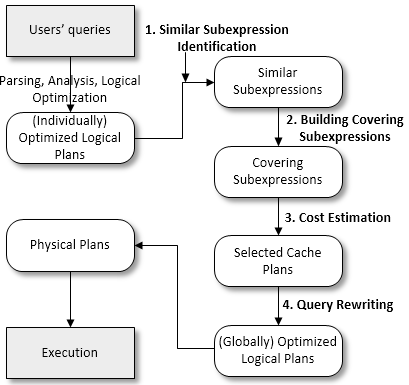
\includegraphics[scale=0.7]{figures/phases_mqo}
   	\caption{Proposed architecture.} 
   	\label{fig:phases_mqo}
\end{figure}

\textbf{Phase 1: Similar subExpressions(SEs) identification}\\
The goal of this phase is to quickly identify all potential sharing opportunities - the Similar Subexpressions (SEs). We compute an \emph{operator fingerprint} for each operator in each logical plan and store it in a fingerprint table. If two operators (and its descendants) have the same fingerprint then we call them similar subexpressions. We will discuss this technique in Section \ref{sec:common_sub}. Found similar subexpressions represents the potential candidates for building covering subexpressions (CEs) in the next phase.

\textbf{Phase 2: Building Covering SubExpressions}\\
Given the sets of SEs, the optimizer first tries to eliminate bad candidates for sharing with the help of cardinality and cost estimation. In this phase, some heuristics are applied to quickly reduce the solution space. Then for each set of SEs, we construct a CE that covers the computation of those expressions. Some CEs are dependent on other CEs, thus CEs are put into groups (classes). Some CEs might become \emph{cache plans} after the cost-based optimization in phase 3.

\textbf{Phase 3: Cost-based optimization}\\
This phase achieves the objective of selecting the best combination of CEs which then become \emph{cache plans}, taking into account the memory constraints and the cost of the caching operation. By using our cost estimation, each CE in previous phase will be assigned a weight and a profit. Finding the best \emph{cache plans} is the most important materialization of our idea to achieve high performance work sharing. We model the challenge such that solving it is equal to solving the Multiple Choice Knapsack problem.

\textbf{Phase 4: Query rewriting}\\
Finally, the input queries are rewritten in which the cache plans are employed. This step involves some basic query transformations on the original queries.

%%%%%%%%%%%%%%%%%%%%%%%%%%%%%%%%%%%%%%%%%%%%%%%%%%%%%%%%%%%%%%%%%%%%%%%%%%%%%%%
\subsection{Common subexpression identification}
\label{sec:common_sub}
The goal of this phase is to quickly identify all potential sharing opportunities in a query and among different queries. The input of this phase is a set of logical plans that are already parsed, analyzed and optimized individually. A logical plan is the internal form representing a query. It is a tree with nodes are logical operators supported by the execution engine. Each operator has its own attribute(s) (filter predicate, project columns, joining condition, etc.).

Our optimization process starts with the optimized logical plans (right before being transformed into physical plans) as the input. Note that we simplified the problem by only focusing on the locally optimal query plans that can derive globally better ones. The first reason is that all queries are already optimized by the same techniques (for example the rule-based optimizer) and usually, the selection and projection operators are pushed to the relations as close as possible. We want to quickly obtain and identify the potential sharing opportunities without paying too much the cost of taking into consideration each single generated logical plan for each query as in \cite{zhou2007efficient}. Keeping that in mind, it is the target of this step to quickly identify and produce reasonable good candidates.

We begin with finding the similar subexpressions in the trees. As being discussed in Section \ref{sec:problem}, we need to strike a balance between (low) memory utilization and (high) benefits from caching. Considering a query has only selection and projection operators, then the higher the node in that tree is, the more selective (less output data) it will be. In other words, some SEs can be safely eliminated from consideration because sharing (caching) them is always worse than some others. However, we may have multiple options if the tree contains one of the following operators: union, cartesian product and join. They are the operators that could possibly produce many output data, even more than the input. Such operators are classified into the \emph{cache-unfriendly operators} group. The rest are \emph{cache-friendly operators} (Filter, Project, Sort, Limit, etc.). Going back to the example in Section \ref{sec:problem}, because SE2, SE3 and SE4 contains only \emph{cache-friendly operators}, we stop looking at the smaller subexpressions for more sharing possibilities. SE1, however, has one \emph{cache-unfriendly operator} - Join. Then we can either select this candidate (SE1) or the 2 smaller ones (SE2 and SE3). We may not be able to immediately conclude which SE is better to share. It depends on multiple criteria (how much we can save in each case, how much data each produces and the memory available, etc.). Potential options are: $\{SE1, SE2, SE3, (SE2, SE3)\}$.

We use the \emph{operator fingerprints} as a technique to detect the similar subexpressions. We first describe how to compute it and how to produce only the ``good" SE candidates. The fingerprint $FP(u)$ of an operator $u$ is computed by:
\[FP(u)= h(H(u) | Sort(FP(u.lchild), FP(u.rchild))) (1)\]
where $h$ is a robust hash function (for example SHA256) and 
\[H(u)=
\begin{cases}
 & h(u.label),\ u= \{Filter, Project\}\\ 
 & h(u.label, u.attributes)),\ otherwise
\end{cases} (2)\]

Node $u$ in the operator tree has its label $u.label$ (operator name) and attributes $u.attributes$ (filter predicate, projection columns, joining conditions, etc.). The $Sort$ in (1) ensures the isomorphic property, for example $TableA\ JOIN\ TableB$ and $TableB\ JOIN\ TableA$ are two isomorphic expressions. If $u$ is a binary node, we have $u.lchild$ and $u.rchild$ as the left and right child. If $u$ is a unary node or a leaf node, (1) will become $FP(u)= h(H(u), FP(u.child))$ and $FP(u)= h(H(u))$ respectively. Note that the fingerprint of a node (an operator) is computed after computing fingerprint of its child(s). Two operators (and its descendants) have the same fingerprint then we call them similar subexpressions. They must have the same tree structure and property. Treating the Filter and Project operations differently in (2) allows us to identify SEs having different filtering predicates and projections. In phase 2, they can be transformed into equivalent expressions sharing a common subexpression. For instance $e1 = Filter_{a>10}(x)$ and $e2 = Filter_{b<30}(x)$ are similar subexpressions, then $e1, e2$ can be transformed into $Filter_{a>10}(Filter_{a>10\ \cup \ b < 30}(x))$ and $Filter_{b<30}(Filter_{a>10\ \cup \ b < 30}(x))$ without changing the expression's result.

Now that we have a mean to compare two operator trees, algorithm \ref{sec:common_sub_alg} searches for SEs among a set of trees while avoid producing worse candidates.

\begin{algorithm}
	\caption{Build hash tree}\label{sec:buildht_alg}
	Input: a logical plans (tree)\\
	Output: HashMap[node, fingerprint]
	\begin{algorithmic}[1]
		\Procedure{$BuildHashTree([T])$}{}
		\State $HT:\{(node, fingerprint)\}=$ empty hash tree
		\For{each node $u$ in $T$}
			\State compute fingerprint $opFT$ for $u$ using (1) and (2)
			\State put $(u, opFT)$ into $HT$
		\EndFor
		\State \Return  $HT$
		\EndProcedure
	\end{algorithmic}
\end{algorithm}

\begin{algorithm}
\caption{Identify similar subexpressions}\label{sec:common_sub_alg}
Input: Array of logical plans (trees)\\
Output: List of SEs put together in group
\begin{algorithmic}[1]
\Procedure{$IdentifySEs([T_{1}, T_{2}, ... T_{N}])$}{}
\State $FT:\{(fp, [nodes])\} =$ empty fingerprint table
%\State $common\_sub\_expressions = \{\}$
\For{each tree $T_{i}, i = 1..N$}
	\State$HT(i) = BuildHashTree(T_{i})$
	\State $AllowedMatching = True$	
	\For{each node $u$ in $T_{i}$ follow the DFS traversal}
		\State $opFP = HT(i)(u)$
		\State $IsMatched = FT$ contains $opFP$
		\If {$AllowedMatching$}
				\State Add $(opFP, u)$ entry to $FT$
		\EndIf
		\State $AllowedMatching = True$	
		\If {$IsMatched$ $AND$ the tree rooted at u does not has cache-unfriendly operator}
			\State Stop the search on u's descendants
		\ElsIf {$IsMatched$ $AND$ the tree rooted at u has cache-unfriendly operator $AND$ $u$ is cache-friendly operator}
			\State $AllowedMatching = False$	
		\EndIf		
	\EndFor
	
\EndFor
\State remove any entries (fp, [nodes]) in FT that has length(nodes) = 1
\State \Return  $FT$
\EndProcedure
\end{algorithmic}
\end{algorithm}

By using the expression (1) and (2), algorithm \ref{sec:buildht_alg} builds a HashTree for each input tree (line 4) of algorithm \ref{sec:common_sub_alg}. Algorithm \ref{sec:buildht_alg} just shows the simplified pseudo code. (Dynamic programming can be applied to save the computations in the for loop). A single fingerprint table (line 2) is used for tracking the matches. Trees with the same fingerprint (same key) will be put in the same group. Following the depth-first-search, each tree and its \emph{operator fingerprint} are added to the fingerprint table (line 10). As being discussed, if we encounter a match on a tree having only cache-friendly operators, then we can safely skip the search on the descendants (line 13 and 14). A group of SEs is detected whenever that group has 2 or more SEs (line 20). Algorithm \ref{sec:common_sub_alg} has O(N*M) complexity where N is the number of trees and M is the average number of nodes per tree.
%%%%%%%%%%%%%%%%%%%%%%%%%%%%%%%%%%%%%%%%%%%%%%%%%%%%%%%%%%%%%%%%%%%%%%%%%%%%%%%

%%%%%%%%%%%%%%%%%%%%%%%%%%%%%%%%%%%%%%%%%%%%%%%%%%%%%%%%%%%%%%%%%%%%%%%%%%%%%%%
\subsection{Building Covering SubExpression}
\label{sec:covering_subexpression}
We identified the potential sharing candidates (SEs) from the input queries, it is the goal of this phase to build the covering subexpressions (CEs) that are the ``covering" computations. Given the sets of SEs, the optimizer first tries to eliminate obviously bad candidates for sharing with the help of cardinality and cost estimation described in Section \ref{sec:cardinality}. Then for each set of SEs, we construct a single CE to produce all common sharing tuples for the consumers (all SEs in that set). Some CEs might become \emph{cache plans} after the cost-based optimization in phase 3. 

In this paper, we define the \emph{cache plan} as the materialization for our work sharing idea. A \emph{cache plan} is a CE defining the result of a materialized view. In other words, cache plans can be seen as temporary views in RDBMSes and to be materialized in RAM. In our work, \emph{cache plans} (selected CEs) will be executed only once and the result is materialized in RAM so that it could be reused multiple times to achieve work sharing. When a query executes, the engine searches in the distributed memory cache to determine whether the results already exists. If yes, it retrieves the result instead. If no, it executes, return the results as output and store them back to the memory cache.

To simplify the problem, we consider the case where only one group of n SEs was identified among the input queries. That means a CE can be built to cover those expressions. We first compare the cost between two approaches: with and without our optimization. We use the notation $C_{E}^{se}$ and $C_{E}^{ce}$ to denote the executing costs of SE $se$ and CE $ce$. $C_{W}^{ce}$ and $C_{R}^{ce}$ are the costs of materializing (writing) the result of CE $ce$ to RAM and retrieving (reading) it back. $C_{COMP}^{se}$ indicates the cost of using the CE to answer the SE $se$.

Given a group of n SEs detected in phase 1, the cost of executing them without optimization can be computed by summing all individual executing costs: $C = \sum _{i=1}^{n}C_{E}^{se_i}$. In contrast, by building a CE and use it as a \emph{cache plan}, this cost becomes: 
$C^* = C_{E}^{ce} + C_{W}^{ce} + \sum _{i=1}^{n}(C_{R}^{ce} + C_{COMP}^{se_i})$. 
CE will be executed and materialized to RAM once. Then the result is read back to answer each individual SE. Only when $C^* < C$, caching brings some benefit in reducing the total job's running time. $C_{E}^{se}$, $C_{E}^{ce}$ and $C_{COMP}^{se_i}$ can be estimated by using cost estimation. $C_{W}^{ce}$ is proportional to the cache size of $ce$, which can be estimated using cardinality estimation. $C_{R}^{ce}$, the cost of reading the cached result of $ce$, is expected to be relatively small. We define the profit $P = (C^*-C)$ which is the profit of using a $ce$ as the cache plan.

%%%%%%%%%%%%%%%%%%%%%%%%%%%%%%%%%%%%%%%%%%%%%%%%%%%%%%%%%%%%%%%%%%%%%%%%%%%%%%%
\subsubsection{CE construction}
\label{sec:ce-construction}
A CE will be built for each group of SEs. Obviously, for SEs that are actually identical expressions, the CE to be built is exactly the same as the SE. Otherwise, we have to apply some transformations on the SEs. The CE is constructed top-down by OR-ing the filtering predicates and combining the projection columns in the SEs. By doing so, the CE could ``cover'' all records required by its consumers. We also remove duplicated predicates to simplify the operators. Figure \ref{fig:covering} illustrates an example of building the covering subexpression for 2 simple SEs. Traversing top-down 2 trees at the same time, whenever projection or filering operators are encountered, we combine their attributes.

\begin{figure}[!htb]
	\centering
	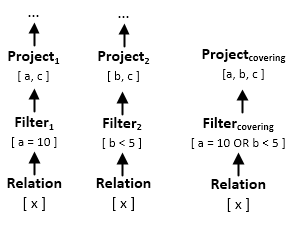
\includegraphics[scale=0.75]{figures/covering}
	\caption{Building covering subexpression example. The first and second trees are two SEs. The third tree is the CE}
	\label{fig:covering}
\end{figure}
%%%%%%%%%%%%%%%%%%%%%%%%%%%%%%%%%%%%%%%%%%%%%%%%%%%%%%%%%%%%%%%%%%%%%%%%%%%%%%%


%%%%%%%%%%%%%%%%%%%%%%%%%%%%%%%%%%%%%%%%%%%%%%%%%%%%%%%%%%%%%%%%%%%%%%%%%%%%%%%
\subsubsection{Pruning bad SEs}
\label{sec:se-prune}
The size of the \emph{cache plans} not only affects the memory occupation but also brings materializing costs. Intuitively, good candidates of \emph{cache plans} are those satisfy the memory constraint while (1) have high frequent of use and/or (2) are expensive to (re)compute, for example producing small amount of output while reading and computing a large amount of input data. Thus, cheap SEs (fast to compute) and heavy SEs (their output exceeds the memory constraint) should be eliminated early from consideration of building the CE. We rather compute them from scratch than just gain a small benefit while paying a big cost in caching a large amount of data. The cost and cardinality estimation we propose in the next section is used to estimate the execution cost and output size of a query.

%%%%%%%%%%%%%%%%%%%%%%%%%%%%%%%%%%%%%%%%%%%%%%%%%%%%%%%%%%%%%%%%%%%%%%%%%%%%%%%
%%%%%%%%%%%%%%%%%%%%%%%%%%%%%%%%%%%%%%%%%%%%%%%%%%%%%%%%%%%%%%%%%%%%%%%%%%%%%%%

%%%%%%%%%%%%%%%%%%%%%%%%%%%%%%%%%%%%%%%%%%%%%%%%%%%%%%%%%%%%%%%%%%%%%%%%%%%%%%%
\subsection{Cost-based optimization}
\label{sec:cbo}
%%%%%%%%%%%%%%%%%%%%%%%%%%%%%%%%%%%%%%%%%%%%%%%%%%%%%%%%%%%%%%%%%%%%%%%%%%%%%%%
\subsubsection{Cardinality and cost estimation}
\label{sec:cardinality}
We design a cardinality and cost estimator to estimate the query's output size and execution cost. Just as traditional work, the system analyzes relational operators and uses some pre-computed statistics data of the input tables.

Computing the query's output size mainly relies on the statistics data, which are computed in 2 levels: relation and column. In relation level, the system obtains the number of records and average record size. In more detail level - column, the system collects the min, max, the cardinality and builds an equi-width histogram for each column. The output size of each operator is estimated under the uniform distribution assumption. 

Although simple, we just want a good estimation to avoid obviously bad plans. More complex histogram techniques could be used to improve the estimation accuracy.


We focus on the CPU, disk I/O and network costs in estimating the total execution cost of a query because they are the three most dominant ones. Those costs are the results of the multiplication between the pre-defined constants and the estimated number of records.




%%%%%%%%%%%%%%%%%%%%%%%%%%%%%%%%%%%%%%%%%%%%%%%%%%%%%%%%%%%%%%%%%%%%%%%%%%%%%%%


%%%%%%%%%%%%%%%%%%%%%%%%%%%%%%%%%%%%%%%%%%%%%%%%%%%%%%%%%%%%%%%%%%%%%%%%%%%%%%%
\subsubsection{Cache plans selection}
\label{sec:cbo-o}
Our problem is to select the best combination of CEs to form the \emph{cache plans}. For each \emph{cache plan}, we compute the (profit, weight). Let's call $W$ is the total cache capacity of the cluster. Then our optimization problem is to maximize the $\sum profit$ under a limited memory capacity: $\sum weight \leq W$. This is the knapsack problem and could be solved by many approaches \cite{•}.

The weight is estimated thanks to the cardinality estimation in section \ref{sec:cardinality}. The profit is the cost difference between (1) executing $n$ SEs and (2) executing the \emph{cache plan} and reused in multiple places. The cost of executing individual SEs are $\sum_{i=1}^n SE_i$ apparently. On the other hand, the cost of (2) is the cost of executing the \emph{cache plan} once, materializing the result to RAM and n times * retrieving the cached data. Furthermore, the cost of applying the \emph{extraction plans} in section \ref{sec:query_rewriting} to compensate the CE and the garbage collection effect are also parts of (2).

Then the combination of \emph{cache plans} to maximize the benefit under the memory limit is equivalent to solving the knapsack problem. Thus, we will be able to first select the best CE among different sharing options.
%%%%%%%%%%%%%%%%%%%%%%%%%%%%%%%%%%%%%%%%%%%%%%%%%%%%%%%%%%%%%%%%%%%%%%%%%%%%%%%

%%%%%%%%%%%%%%%%%%%%%%%%%%%%%%%%%%%%%%%%%%%%%%%%%%%%%%%%%%%%%%%%%%%%%%%%%%%%%%%

%%%%%%%%%%%%%%%%%%%%%%%%%%%%%%%%%%%%%%%%%%%%%%%%%%%%%%%%%%%%%%%%%%%%%%%%%%%%%%%
\subsection{Query Rewriting}
\label{sec:query_rewriting}
Now that we selected the best combination of \emph{cache plans}, the last step is to transform the original input queries to use them. First, the execution engine should be noticed that the output of \emph{cache plans} will be materialized in RAM after its execution. Next, the transformation applied on the input queries is the replacement of SEs by the \emph{extraction plans} on top of the \emph{cache plans}. Remember that \emph{cache plans} are the selected covering subexpressions that covers the records for their consumers. We need to re-apply the filtering and projection to assures the output of queries does not change.

For each input query having the SE and employing the cache plan respectively, we build an \emph{extraction plan} that compensates the cache plan such that the output of the extraction plan on top of the cache plan is equals to the output of that SE. The query rewriting in Figure \ref{fig:rewrite} is a simple example illustrating the technique. In more abstract, we build the \emph{extraction plans} by AND-ing the filtering predicates and combining the top projection columns of the SE.

\begin{figure}[!htb]
	\centering
ubstaint	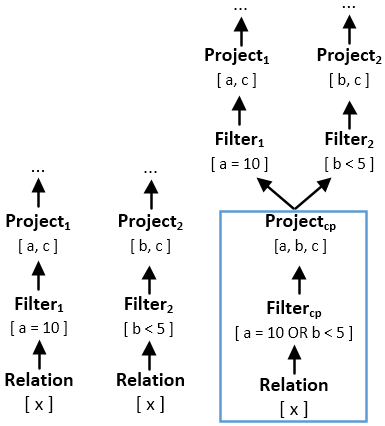
\includegraphics[scale=0.55]{figures/rewrite}
	\caption{Query rewriting example. The tree in rectangle is the cache plan}
   	\label{fig:rewrite}
\end{figure}
%%%%%%%%%%%%%%%%%%%%%%%%%%%%%%%%%%%%%%%%%%%%%%%%%%%%%%%%%%%%%%%%%%%%%%%%%%%%%%%

We next cover in detail the implementation of our system running on Apache Spark and Spark SQL.
%%%%%%%%%%%%%%%%%%%%%%%%%%%%%%%%%%%%%%%%%%%%%%%%%%%%%%%%%%%%%%%%%%%%%%%%%%%%%%%

%%%%%%%%%%%%%%%%%%%%%%%%%%%%%%%%%%%%%%%%%%%%%%%%%%%%%%%%%%%%%%%%%%%%%%%%%%%%%%%
\section{Implementation details}
\label{sec:implementation}
%%%%%%%%%%%%%%%%%%%%%%%%%%%%%%%%%%%%%%%%%%%%%%%%%%%%%%%%%%%%%%%%%%%%%%%%%%%%%%%
\subsection{Apache Spark and Spark SQL overview}
% \label{sec:}
% \input{}
%%%%%%%%%%%%%%%%%%%%%%%%%%%%%%%%%%%%%%%%%%%%%%%%%%%%%%%%%%%%%%%%%%%%%%%%%%%%%%%
%\mytodo{Intro to spark, refer to spark paper: the paradigm, the abstraction, speed, ...}.
In this paper, we adopt an open-source processing engine: Apache Spark. Among the prevalent engines, Spark is proven to bring strong performance due to its in-memory computation nature. It is the first cluster computing engine that leverages the distributed memory abstraction and outperforms Hadoop by up to 20X in iterative applications \cite{zaharia2012resilient}. This motivated us to propose a new in-memory cache-based optimization for cloud environment. Spark SQL is the high level language support running on top of Spark. We present the implementation of our solution in the query optimizer of Spark SQL.

Spark SQL defines an SQL-like high-level language for processing large-scale analytic workloads. The queries expressed in the high-level languages are finally transformed into RDDs as the abstract concept of Spark core engine. Queries written in Spark SQL are in an abstract form: the DataFrames. A DataFrame object represents a \emph{logical plan} to compute a dataset. A logical plan is a tree composed of operators (nodes). Each has operator name (operator type) and attributes (filtering predicates, join columns, etc.). A node could be binary, unary or leaf node that has 2 children, 1 child or zero child respectively.

Catalyst \cite{sparksql} is the query optimizer of Spark SQL. Catalyst focuses on optimizing each single query, while in our approach, a cost-based optimizer is applied to optimize multiple queries together. The rule-based optimizer in Spark SQL defines the rules (constant folding, early filtering, and predicate pushdown, etc.) to produce optimized logical plans. Using the cost model to decide the joining strategies, the optimized logical plans are then transformed to single physical plan for execution. Figure \ref{fig:sparksql_queryplanning} illustrates the internal Spark SQL's architecture, and the modules involved in parsing and generating the various query plans discussed above.

\begin{figure*}[t]
   \centering
   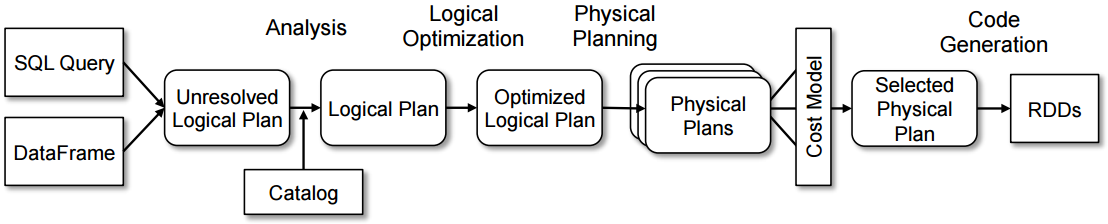
\includegraphics[scale=0.45]{figures/sparksql_queryplanning}
   \caption{Phases of query planning in Spark SQL. Rounded rectangles represent Catalyst trees \cite{sparksql}} 
   \label{fig:sparksql_queryplanning}
\end{figure*}

%%%%%%%%%%%%%%%%%%%%%%%%%%%%%%%%%%%%%%%%%%%%%%%%%%%%%%%%%%%%%%%%%%%%%%%%%%%%%%%
\subsection{Implementation of work sharing for Spark SQL}
\label{sec:plan_implementation}
In Spark SQL, for each individual application, it is possible to indicate which data (DataFrame) to cache in memory. Subsequent data transformation can reuse cached data without the need to recompute it from the lineage. However, Spark applications submitted to a cluster by different clients are totally isolated from each other\cite{zaharia2012resilient}, therefore, sharing across applications is not trivial. To avoid modifying spark's internal architecture principle, we build a centralized Spark SQL server serving requests from multiple users while acting as a single client of cluster. The optimization we proposed is being done at this central Spark SQL server.

In our system, we use the optimized logical plans as the input for the query optimizer. Users have many interfaces to express the data they want in Spark SQL. Logical plan is the one that abstract and unified. The optimized logical plan is the last logical representation of a query before converting it to a physical. If the input queries are similar, looking at the optimized logical plans is the best way to discover the similar parts.

We follow the optimization process of 4 phases discussed in section \ref{sec:caching}. Operator fingerprints are computed to identify all similar subexpressions in the first phase. Phase 2 and phase 4 require some query transformations. We take advantage of the pattern matching feature of scala and the TreeNode library of Catalyst in Spark SQL to rewrite queries. Transforming rules are passed as a function to specify how to transform the trees. Pre-computed statistics data computed in phase 3 are done by launching 2 jobs for each table. The cardinality of each column is estimated using the algorithm HyperLogLog.
%%%%%%%%%%%%%%%%%%%%%%%%%%%%%%%%%%%%%%%%%%%%%%%%%%%%%%%%%%%%%%%%%%%%%%%%%%%%%%%

%%%%%%%%%%%%%%%%%%%%%%%%%%%%%%%%%%%%%%%%%%%%%%%%%%%%%%%%%%%%%%%%%%%%%%%%%%%%%%%
\section{Experimental Evaluation}
\label{sec:evaluation}
%Khoa
We now present experimental results to evaluate the effectiveness of our prototype on Spark and Spark SQL. First, we focus on a detailed analysis of caching efficiency with respect to simple queries, that just focus on individual operators. We want to convey the sense of the effectiveness of data caching in work sharing system to the readers. We then proceed with a general overview of the performance gains achieved with our optimizer, using the standard TPC-DS benchmarking. The efficiency of our cost-model is also evaluated experimentally.

%%%%%%%%%%%%%%%%%%%%%%%%%%%%%%%%%%%%%%%%%%%%%%%%%%%%%%%%%%%%%%%%%%%%%%%%%%%%%%%
\subsection{Experimental setup}
\label{sec:setup}
%\include{setup}
We run the micro-benchmark on cluster consisting of 14 worker nodes. Each node has 6 GB RAM of which 3 GB is used for caching data. The data set is stored in HDFS (replication = 3) in Parquet and CSV format. 

For the micro-benchmark, the data sets are randomly generated. The schema of data set is as follows: \texttt{(Name: str[20], Age: int, Dep: int, Desc1: str[100], Desc2: str[200])}. The Age column follows uniform distribution in the range [1, 100] so that we can later adjust the input/output ratio. The data sets have various number of records and sizes: 10M records (3 GB), 30M (9 GB), 50M (15 GB), 80M (24 GB), 100M (30.6 GB), 130M (40 GB), 150M (46 GB) and 200M (61 GB).

For the macro-benchmark, we use TPC-DS benchmark library developed by Databricks for Spark and Spark SQL \cite{sparksqlperf}. The scaling factor is set to 10, 30, 50 and 100.

Before running each test, we clear the operating system's buffer cache to obtain more accurate result. Each single test is run 3 times and we take the average.

%%%%%%%%%%%%%%%%%%%%%%%%%%%%%%%%%%%%%%%%%%%%%%%%%%%%%%%%%%%%%%%%%%%%%%%%%%%%%%%
%%%%%%%%%%%%%%%%%%%%%%%%%%%%%%%%%%%%%%%%%%%%%%%%%%%%%%%%%%%%%%%%%%%%%%%%%%%%%%%
\subsection{Micro-benchmarks}
\label{sec:micro}
In this Section, we evaluate our system through a series of experiments on simple queries. We focus on just simple ones to emphasize the benefits of caching as a function of the particular operators involved in each query. For simplicity, we consider workloads composed by two queries only, and compute the running time of the Spark jobs associated to each query, with and without our cache-based multi-query optimization mechanism. Overall, our results indicate:

\begin{itemize}
	\item The format of input files matters the increase of job's performance.
	\item Roughly 50\% and 30\% improvement in aggregate query latencies for CSV and Parquet files respectively.
	\item Memory utilization is minimized.
\end{itemize}

We use the following notation:
\begin{itemize}
	\item R\_Job1, R\_Job2: job execution times, with no caching
	\item R\_Job1*, R\_Job2*: job execution times, with caching
	\item M\_R: Total memory utilization, in Bytes
	\item M\_D: Total disk utilization, in Bytes. This metric accounts for data that does not fit in RAM, and is spilled to disk by the Spark caching mechanism.
	\item M: total memory caching capacity
	\item I: input size of the dataset, in terms of records.
\end{itemize}

We first examine Filter and Project operations because they appear very frequently in data analysis, and are usually pushed as close as possible to the input by traditional query optimization techniques. Then, we consider the join operation that involves shuffling data across the network.

\subsection{Filter-based queries}
The two queries are described by the logical plans depicted in Figure \ref{fig:query1_plans}. The top left and top right logical plans indicate that the two queries we consider read data from the same input relation, then apply a filter operation with two different predicates. The logical plan displayed at the bottom of the Figure is the result output by our multi-query optimizer: Job1* first reads the data from the input relation, then applies a Filter operator, with a combined predicate. Next, Job1* caches the filtered data and finally applies its own filter predicate to produce the output. The second job Job2*, reads directly its input data from the cache.

\begin{figure}[htbp]
   \centering
   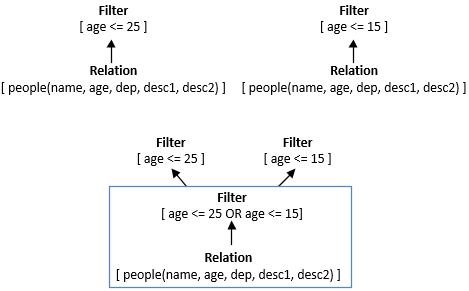
\includegraphics[scale=0.5]{figures/query1_cacheplan}
   \caption{Query and Cache plan for Filter-based queries.} 
   \label{fig:query1_plans}
\end{figure}

Next, in Figure \ref{fig:query1}, we show the individual and aggregate query latencies, with and without our optimization. We also show the impact of the input data format, considering both Parquet and CSV input files.

\begin{figure}[!htb]
	\centering
	\subfigure[Parquet]{
   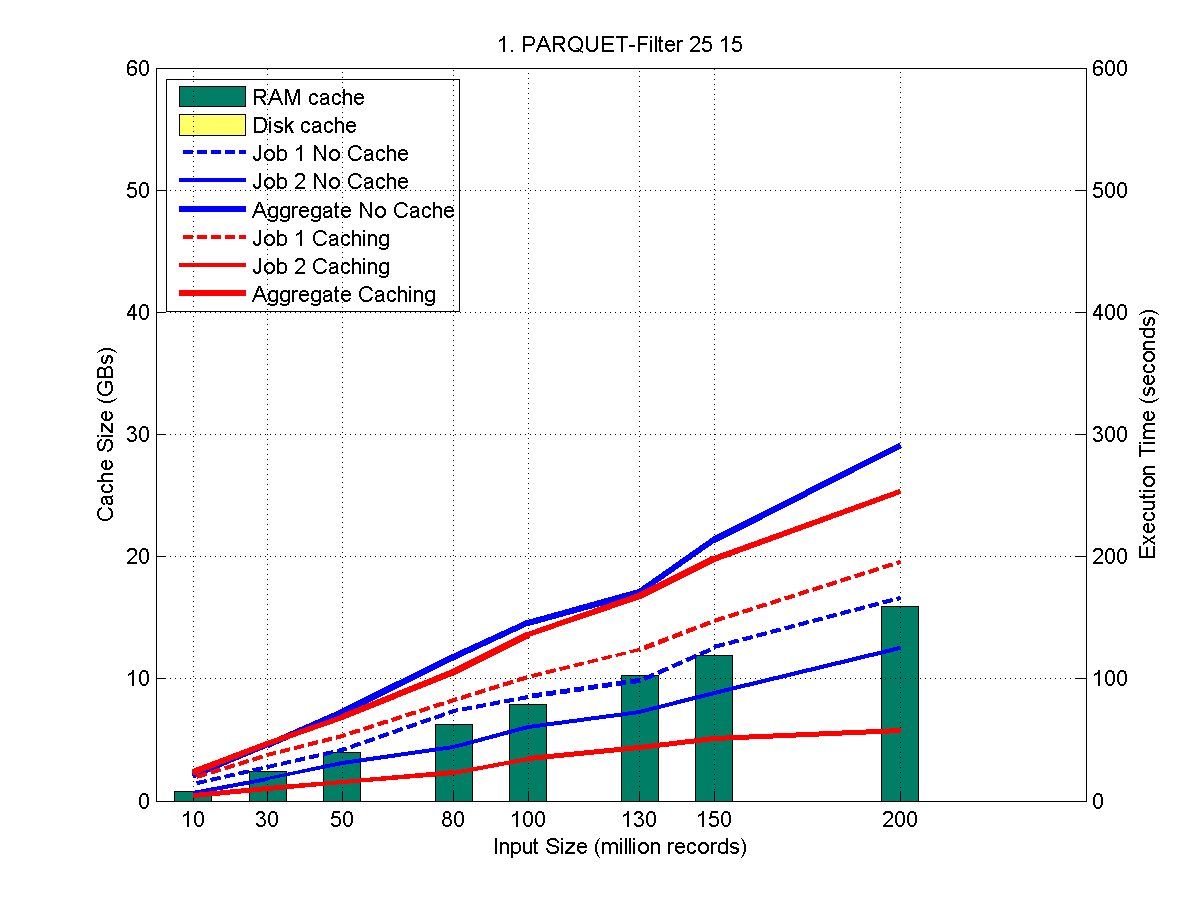
\includegraphics[scale=0.35]{figures/query1_parquet}
   \label{fig:query1_parquet}}

  	\subfigure[CSV]{
   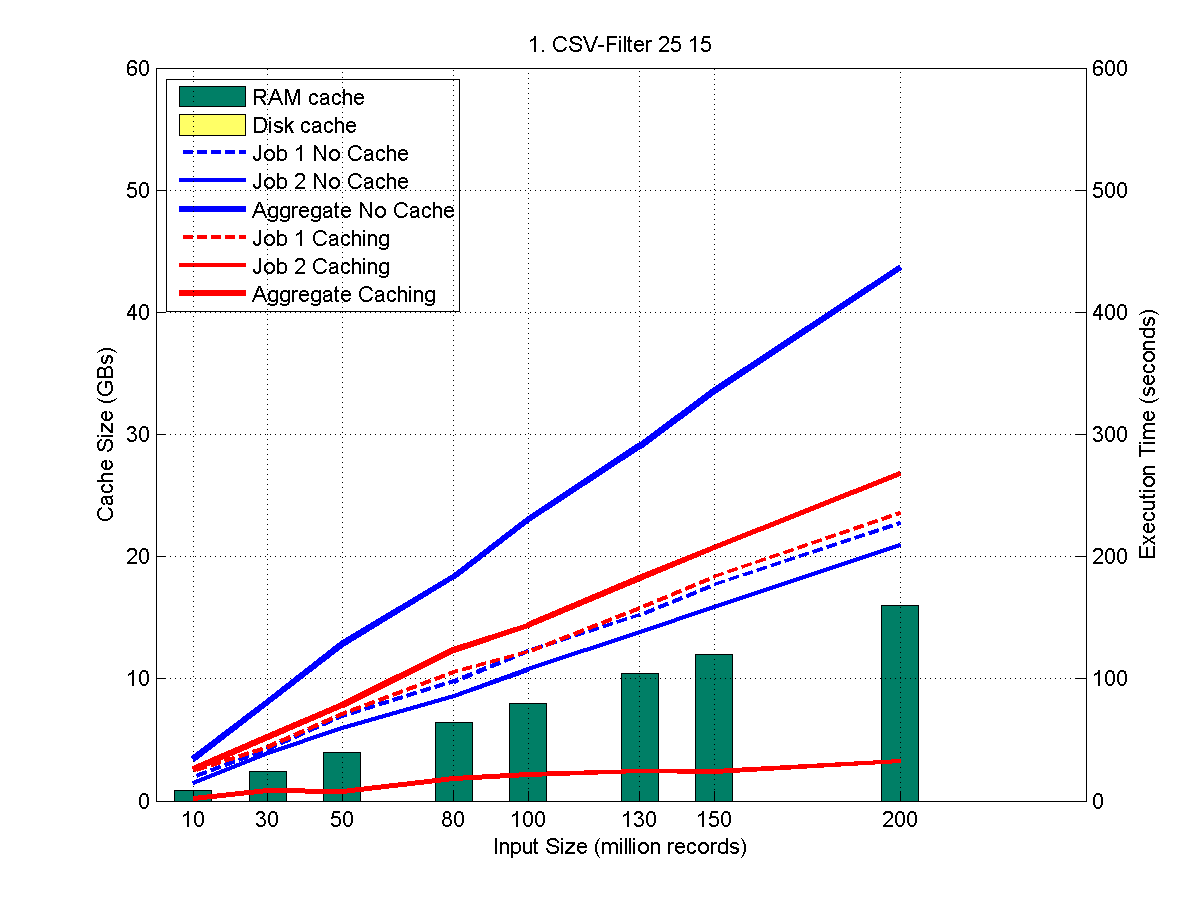
\includegraphics[scale=0.35]{figures/query1_csv}
   \label{fig:query1_csv}}

   \caption{Filter-based queries, query latencies and memory utilization.}
   \label{fig:query1}
\end{figure}

The first set of results indicate the multi-query optimizer works as expected: for both Parquet and CSV input format, the aggregate query latency for the two jobs is shorter with caching optimization. In details, we notice that Job1* runs slower than Job1: this is attributed to the cost of the caching operation. However, the difference in runtime between Job1* and Job1 is not the same for the case Parquet (noticeable different) and CSV (somehow equals). Additionally, the execution time of Job2* (which involves reading data from cache then writing data to disk) for both formats shows different pattern: when data is in Parquet format, Job2* benefits less from caching.

The cache size is roughly 25\% of the size of input data, for both the Parquet and CSV case. Our multi-query optimizer uses only 1/3 of the caching capacity (25\% of 200M records costs 16GB of cache size, which totals 45GB in our system).

Next, we consider a different set of filtering conditions, which are more stressful with respect to memory utilization. The queries we consider are less selective than the ones presented above, with filtering predicates as follows: \texttt{age <= 50} and \texttt{age <= 25}. Figure \ref{fig:query1_50} shows query latencies and memory utilization respectively.

\begin{figure}[!htb]
	\centering

	\subfigure[Parquet]{
   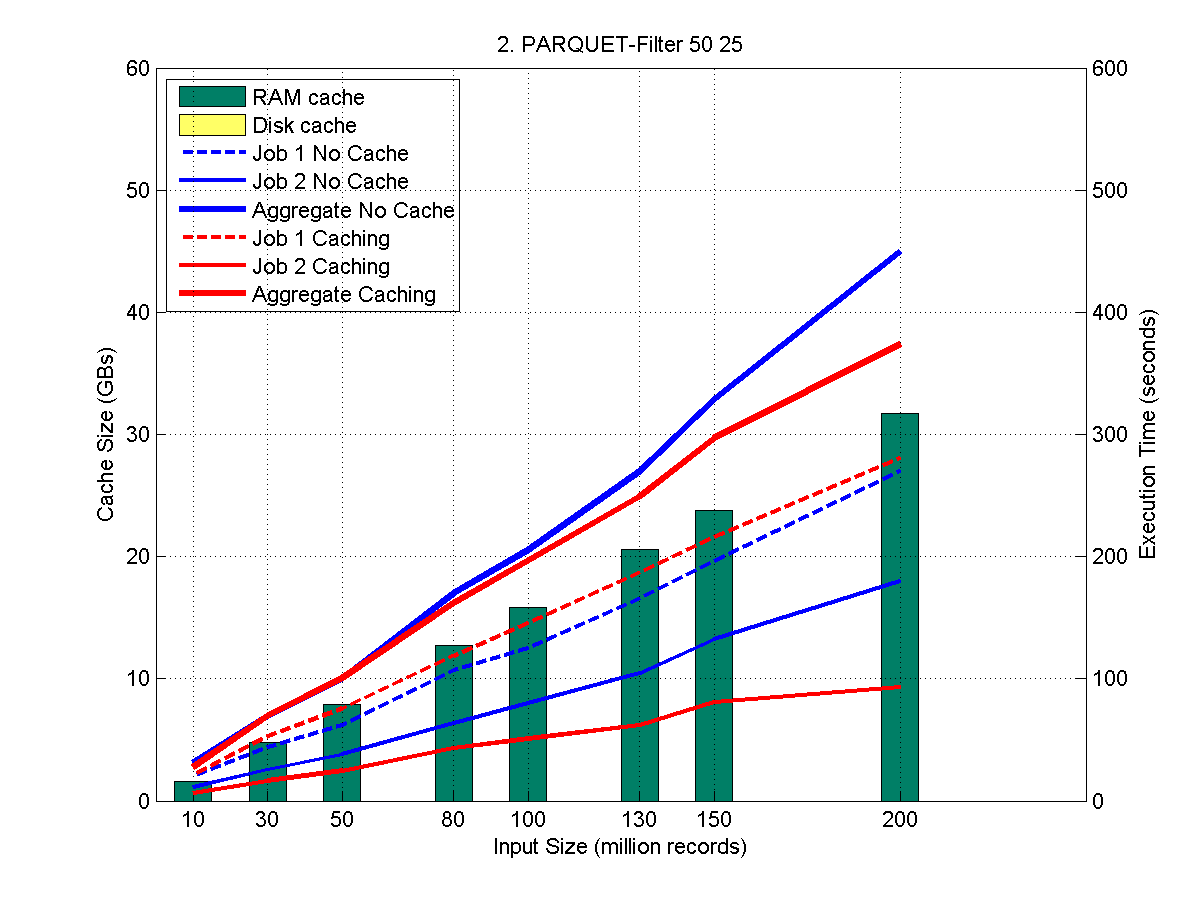
\includegraphics[scale=0.35]{figures/query1_parquet_50}
   \label{fig:query1_parquet_50}}

  	\subfigure[CSV]{
   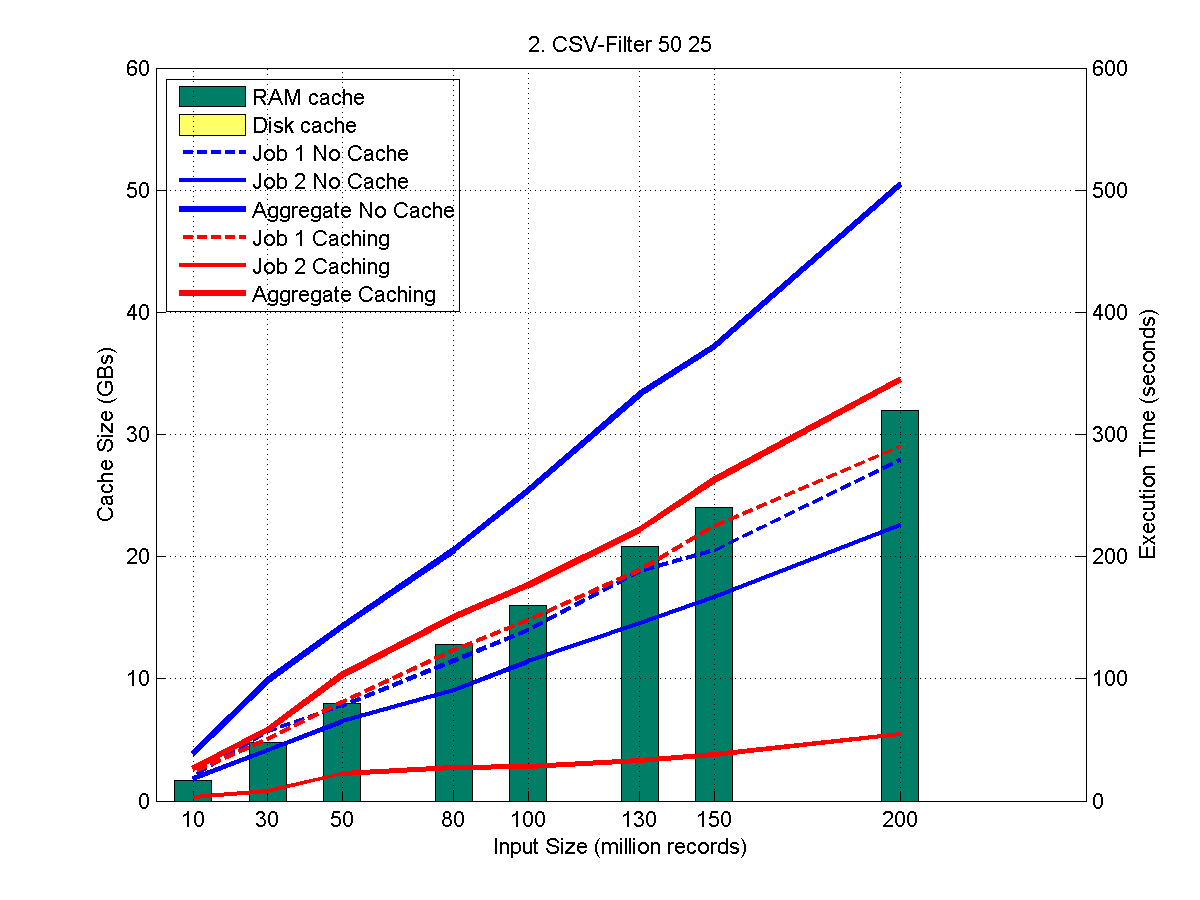
\includegraphics[scale=0.35]{figures/query1_csv_50}
   \label{fig:query1_csv_50}}

   \caption{Filter-based queries, query latencies and memory utilization.}
   \label{fig:query1_50}
\end{figure}

Finally, we consider even less selective predicates, defined as follows: (\texttt{age <= 80} and \texttt{age <= 15}). Figures \ref{fig:query1_80_15} show query latencies and memory utilization. For this set of filtering conditions the optimizer caches a lot of data in Job1, of which very little is useful for Job2: as a consequence, the cost of caching might not be balanced by its benefits. This shows that the amount of performance gain also depends on the cardinalities of expressions.

\begin{figure}[!htb]
	\centering

	\subfigure[Parquet]{
   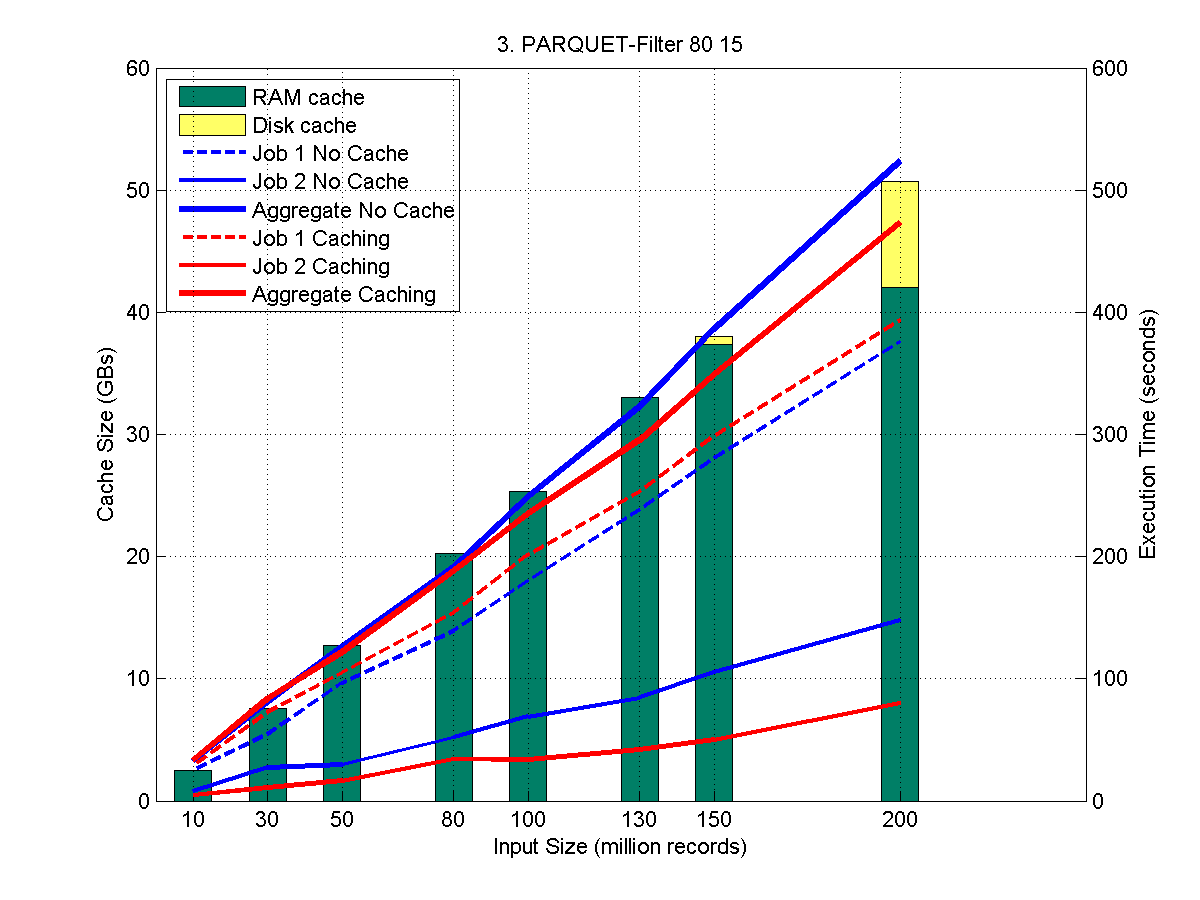
\includegraphics[scale=0.35]{figures/query1_parquet_80_15}
   \label{fig:query1_parquet_80_15}}

  	\subfigure[CSV]{
   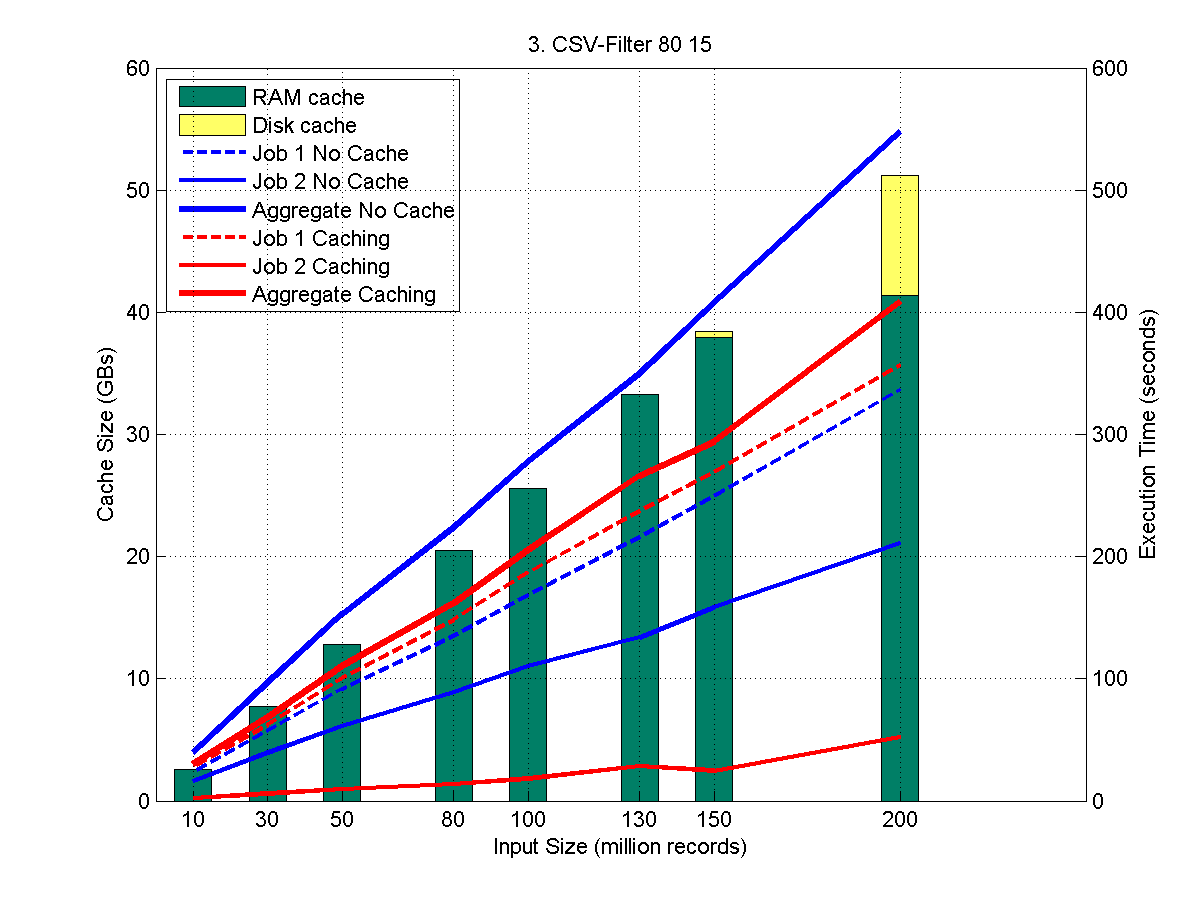
\includegraphics[scale=0.35]{figures/query1_csv_80_15}
   \label{fig:query1_csv_80_15}}

   \caption{Filter-based queries, query latencies and memory utilization.}
   \label{fig:query1_80_15}
\end{figure}

\subsection{Projection-based queries}
Next, we consider simple queries that only perform project operations. Specifically, with reference to the schema of our input data, queries project two attributes: \texttt{desc1:string[100]} and \texttt{desc2:string[200]}.

The original logical plans of the two queries, along with the optimized plan that uses caching are depicted in Figure \ref{fig:query2_plans}.

\begin{figure}[!htb]
   \centering
   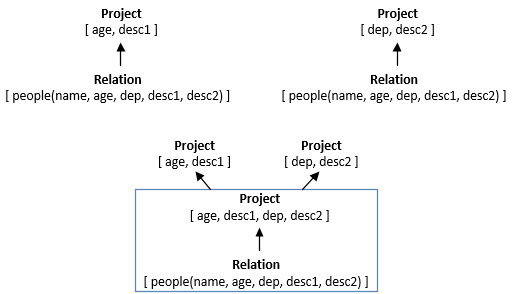
\includegraphics[scale=0.5]{figures/query2_cacheplan}
   \caption{Query and Cache plans for Project-based queries.} 
   \label{fig:query2_plans}
\end{figure}

Next, we present the analysis of the query latencies with and without our optimization, for both Parquet and CSV input data types, in Figures \ref{fig:query2}.

\begin{figure}[!htb]
	\centering

	\subfigure[Parquet]{
   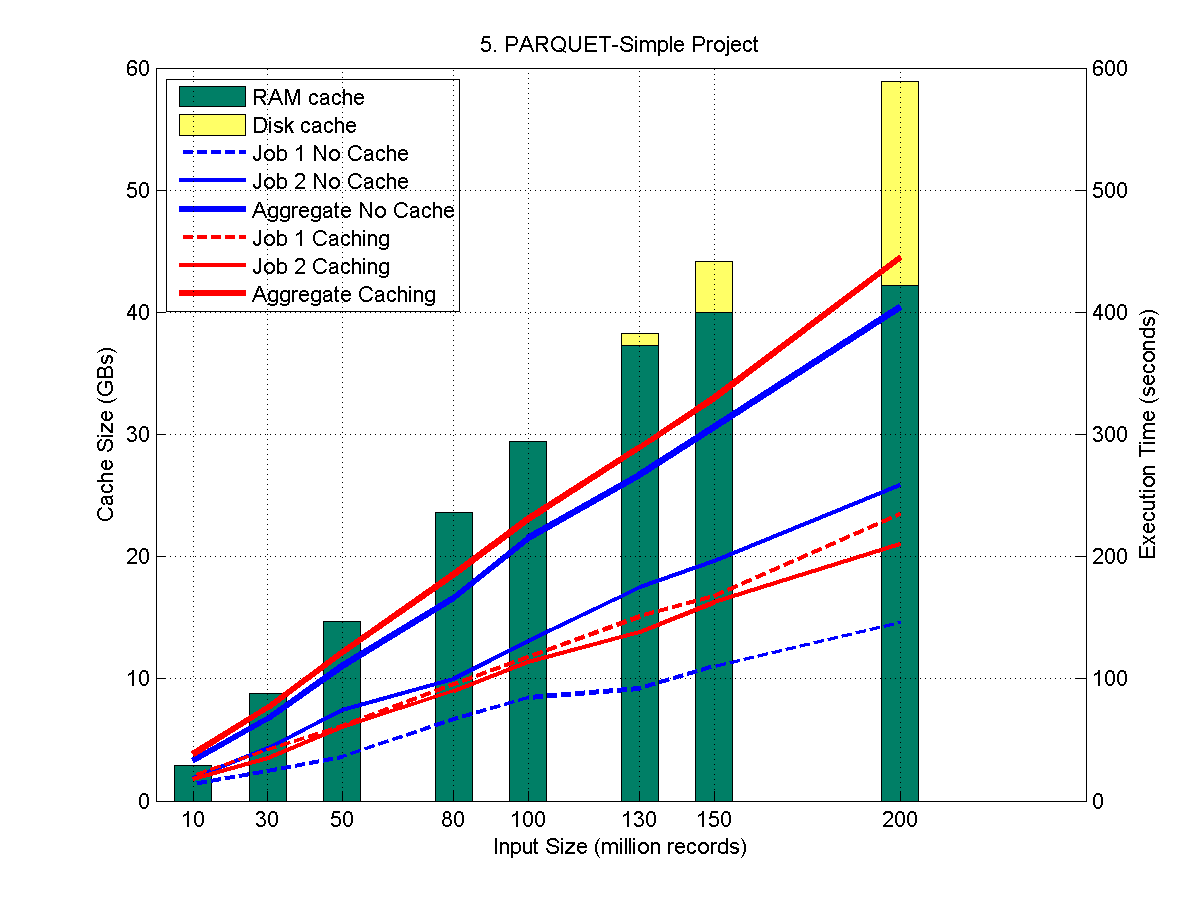
\includegraphics[scale=0.35]{figures/query2_parquet}
   \label{fig:query2_parquet}}

  	\subfigure[CSV]{
   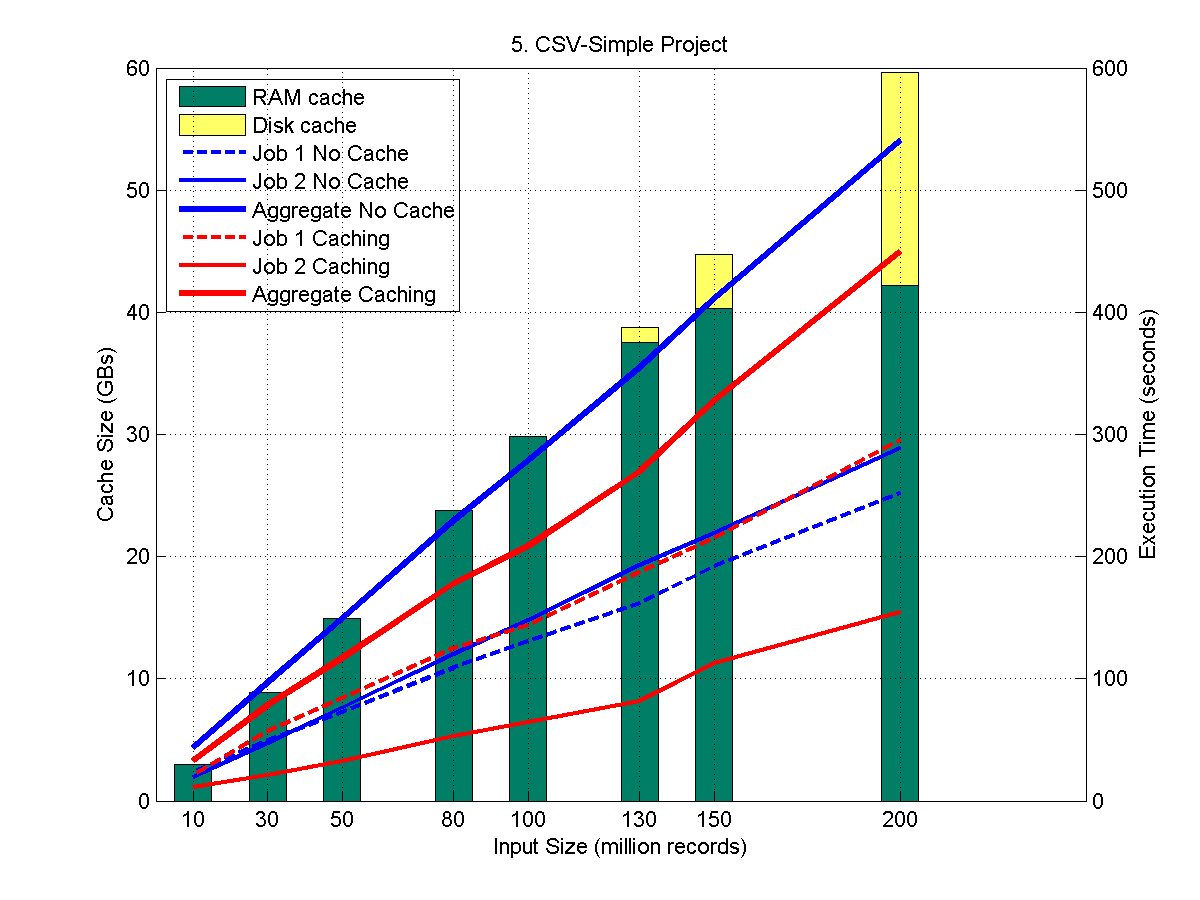
\includegraphics[scale=0.35]{figures/query2_csv}
   \label{fig:query2_csv}}

   \caption{Project-based queries, query latencies and memory utilization.}
   \label{fig:query2}
\end{figure}

Our observations on the results for Project-based queries are as follows. 
When using CSV input data, the benefit of our optimization is clear. Instead, when using the Parquet format, our results indicate little to no benefit in using our optimization. Indeed, Parquet is geared towards columnar data access on disk: as a consequence, the cost associated to cache input data outweighs the benefits of reading two columns from RAM instead of using their disk representations.

\subsection{Projection and Filter based queries}
We now study the impact of our optimization on two queries that mix projection and filters. The logical plans and the optimized plan output by our approach are depicted in Figure \ref{fig:query3_plans}

\begin{figure}[!htb]
   \centering
   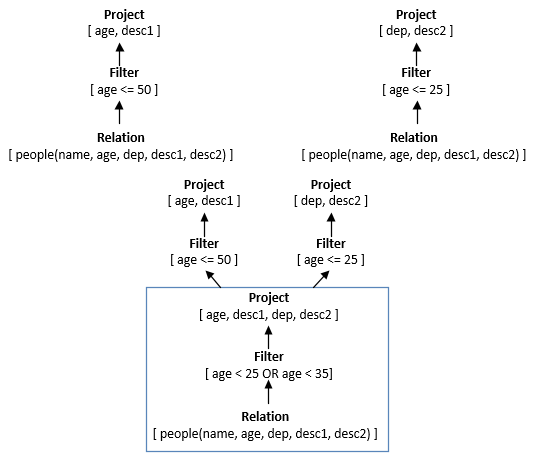
\includegraphics[scale=0.5]{figures/query3_cacheplan}
   \caption{Query and Cache plans for Project and filter based queries.} 
   \label{fig:query3_plans}
\end{figure}

Next, we present the analysis of the query latencies with and without our optimization, for both Parquet and CSV input data types, in Figures \ref{fig:query3}.

\begin{figure}[!htb]
	\centering

	\subfigure[Parquet]{
   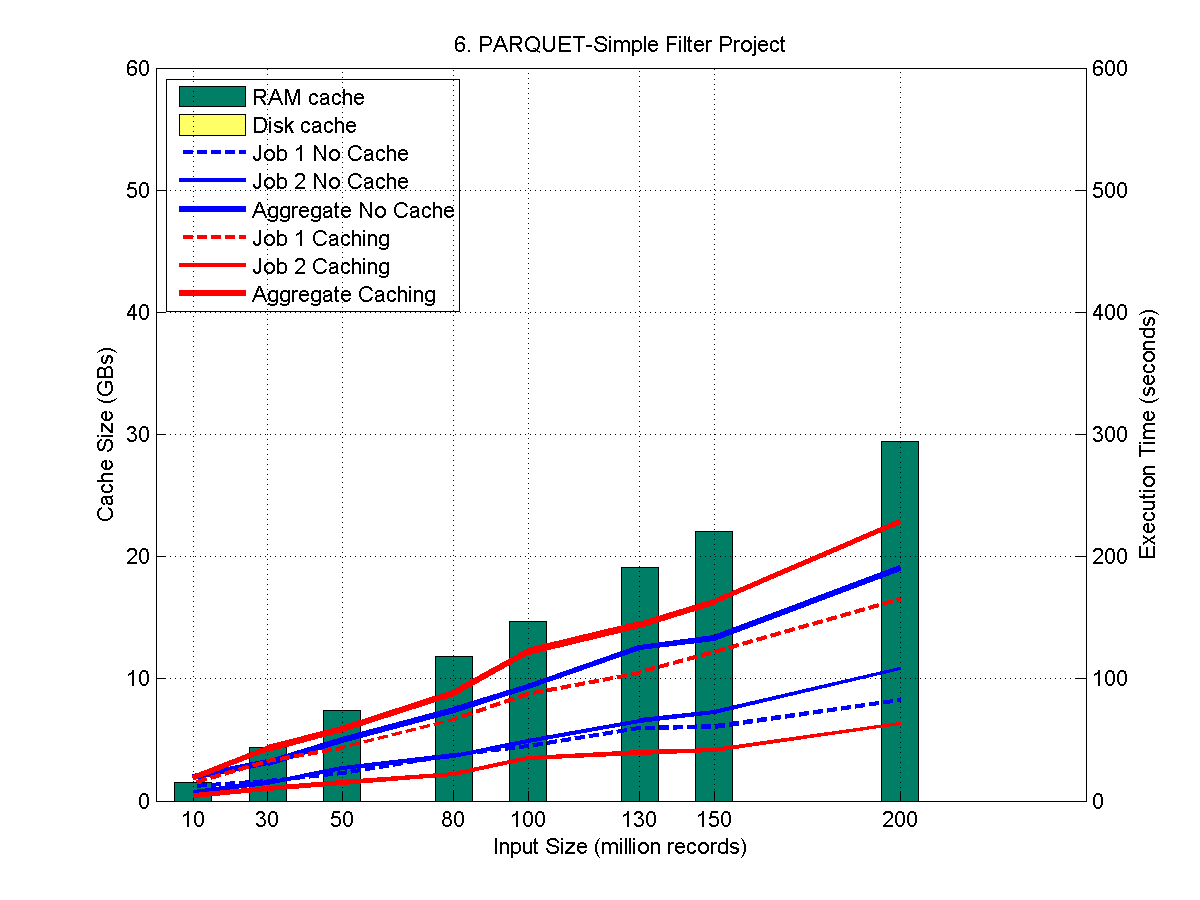
\includegraphics[scale=0.35]{figures/query3_parquet}
   \label{fig:query3_parquet}}

  	\subfigure[CSV]{
   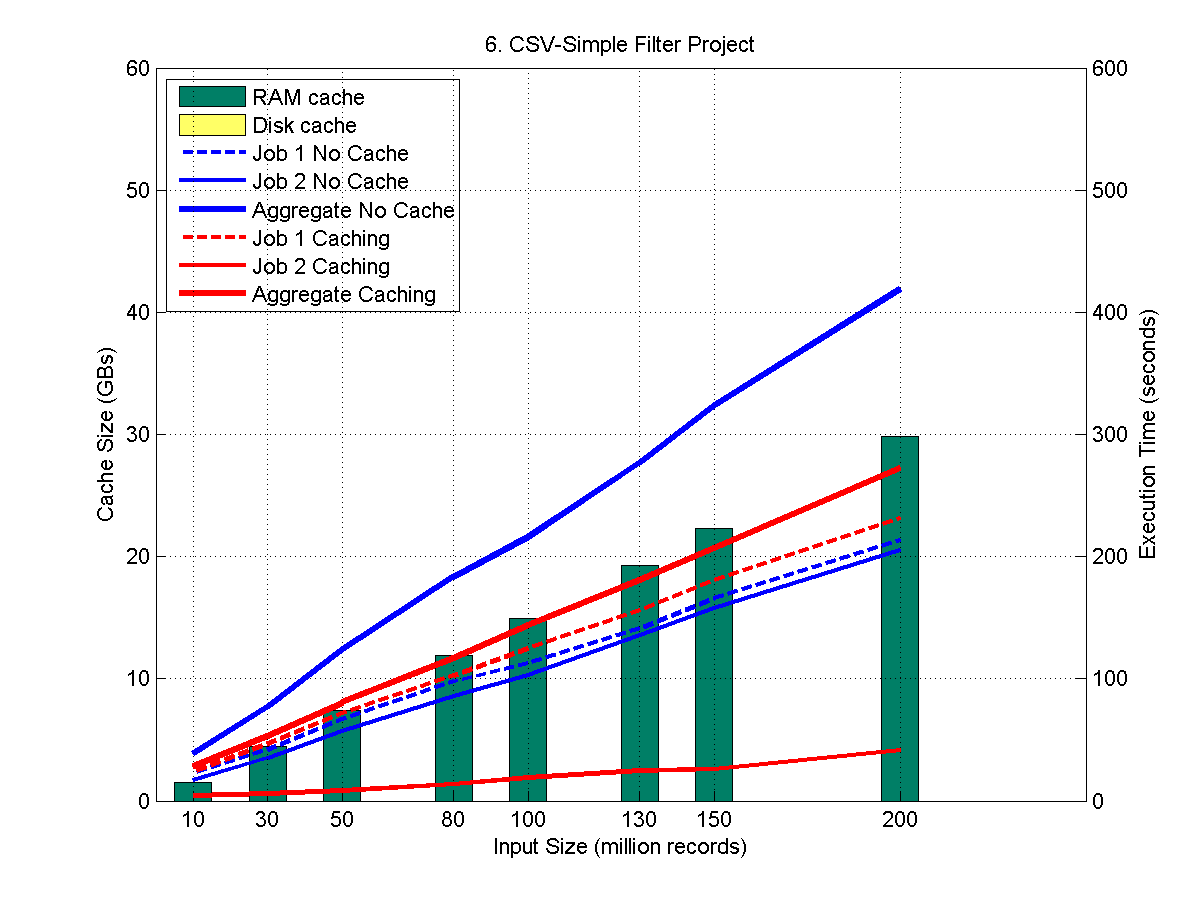
\includegraphics[scale=0.35]{figures/query3_csv}
   \label{fig:query3_csv}}

   \caption{Project-based queries, query latencies and memory utilization.}
   \label{fig:query3}
\end{figure}

Our results indicate that the ``economy'' of our optimization requires a detailed cost-based analysis: in particular, projections on parquet formatted input files do not benefit from caching, and the cost of the cache operation is larger than its benefits.

\subsection{Joining queries}
We now study consider queries that involve costly processing. In particular, ranking data requires ``shuffling'' data over the network and sorting.

%%%%%%%%%%%%%%%%%%%%%%%%%%%%%%%%%%%%%%%%%%%%%%%%%%%%%%%%%%%%%%%%%%%%%%%%%%%%%%%
%%%%%%%%%%%%%%%%%%%%%%%%%%%%%%%%%%%%%%%%%%%%%%%%%%%%%%%%%%%%%%%%%%%%%%%%%%%%%%%
\subsection{Macro-benchmarks}
\label{sec:macro}
We also run the experiment on the TPC-DS queries that are compatible with Spark SQL, developed by the author of Spark and Spark SQL \cite{sparksqlperf}.

%%%%%%%%%%%%%%%%%%%%%%%%%%%%%%%%%%%%%%%%%%%%%%%%%%%%%%%%%%%%%%%%%%%%%%%%%%%%%%%
%%%%%%%%%%%%%%%%%%%%%%%%%%%%%%%%%%%%%%%%%%%%%%%%%%%%%%%%%%%%%%%%%%%%%%%%%%%%%%%
\subsection{Cost model evaluation}
\label{sec:cost}
%%%%%%%%%%%%%%%%%%%%%%%%%%%%%%%%%%%%%%%%%%%%%%%%%%%%%%%%%%%%%%%%%%%%%%%%%%%%%%%

%%%%%%%%%%%%%%%%%%%%%%%%%%%%%%%%%%%%%%%%%%%%%%%%%%%%%%%%%%%%%%%%%%%%%%%%%%%%%%%
\section{Conclusion}
\label{sec:conclusion}
This paper presents a novel idea of applying cache primitives and multi-query optimization means to large-scale distributed systems. Our prototype extends the current Spark SQL's query optimizer and address multiple challenges to achieve high performance work sharing. Scheduling input queries, cache eviction and adaptive cost model could be other dimensions that we could work to improve our system.
%%%%%%%%%%%%%%%%%%%%%%%%%%%%%%%%%%%%%%%%%%%%%%%%%%%%%%%%%%%%%%%%%%%%%%%%%%%%%%%


\bibliographystyle{abbrv}
\bibliography{references}

\end{document}